Cerchiamo ora di ragionare su sistemi più complessi.

Finora non abbiamo studiato molecole in cui fossero presenti doppietti sull'atomo centrale. Per spiegare le geometrie di queste è necessario introdurre la teoria \textbf{V.S.E.P.R.} (Valence Shell Electron Pair Repulsion (Tradotto: repulsione delle coppie elettroniche nel guscio di valenza)), che tiene conto della repulsione esercitata dalle coppie di elettroni. Infatti, essendo cariche dello stesso segno, gli elettroni tenderanno a respingersi fra di loro, per cui le molecole assumeranno delle geometrie tali che questa repulsione sia minima, ovvero quelle che tengono le coppie di elettroni il più lontano possibile tra loro.
\subsection{Coppie singole e coppie di legame}
Per spiegare alcune variazioni su certi angoli di legame si è pensato, ed è realistico, che le coppie di elettroni di legame non siano localizzate su un solo atomo, ma su entrambi quelli legati da tale coppia, e che quindi abbiano più spazio di quanto ne abbiano a disposizione le coppie solitarie, localizzate su un solo atomo. Ne segue che ci sarà diversa repulsione tra coppie di legame e coppie di legame, tra coppie di legame e coppie solitarie e tra coppie solitarie e coppie solitarie.

È ragionevole che due coppie di elettroni non coinvolte nel legame e che si trovano nello stesso atomo si respingano di più di una coppia di elettroni di legame con una solitaria, le quali a loro volta si respingono di più di due coppie di legame.

Di volta in volta dovremo quindi andare a vedere come si dispongono nello spazio tutti gli elettroni, con l'obiettivo di vedere quale possa essere la geometria che permette una minore repulsione.

La conseguenza di ciò è che quando sono presenti coppie solitarie, gli angoli reali differiscono da quelli teorici.
\subsection{Geometrie tetraedriche}
Le coppie solitarie devono comunque stare su un orbitale, quindi nei casi che andremo a osservare sarà comunque necessaria una ibridizzazione di tipo sp$^3$.

\vspace{0.2cm}\textbf{ES.1} $\rm CH_4$ (4 coppie di legame)
    
\vspace{0.2cm}Nel metano la geometria che minimizza le repulsioni è quella tetraedrica, con angoli di legame di 109.5°.

\vspace{0.2cm}\textbf{ES.2} $\rm NH_3$ (3 coppie di legame e una solitaria)

\begin{figure}[H]
    \centering
    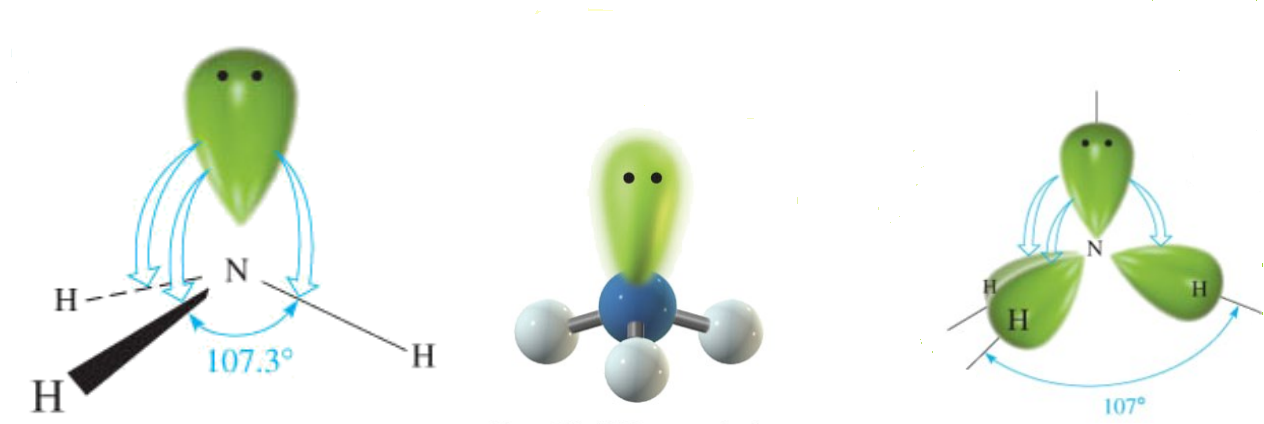
\includegraphics[width=12cm]{immagini/ammoniaca.png}
\end{figure}
    
Secondo il formalismo di Lewis, l'ammoniaca vedeva poste sull'azoto tre coppie di legame dovute ai tre legami con l'idrogeno e una sola coppia solitaria.

Supponiamo che non ci sia stata ibridizzazione e che non ci siano repulsioni elettroniche: in questo caso si osserverebbe che i legami hanno fra loro angoli di 90°, in quanto sarebbero formati dagli orbitali p, che sono perpendicolari tra loro.
    
Se invece ci fosse stata ibridizzazione sp$^3$, ci aspetteremmo angoli di legame di 109.5°.
    
Nei fatti non si osserva né una geometria né l'altra: si osserva una struttura simile a quella tetraedrica, in cui i tre atomi di idrogeno stanno sullo stesso piano mentre l'azoto è sopraelevato rispetto a questo, ma con angoli di 107.8°, circa due gradi in meno.
    
Grazie alla teoria V.S.E.P.R. riusciamo a spiegare questa differenza: la coppia solitaria dell'azoto respinge maggiormente le tre coppie di legame di quanto farebbe un'ipotetica quarta coppia di legame (vedi il metano), e quindi per minimizzare questa repulsione le coppie di legame si devono allontanare di più e di conseguenza l'angolo di legame diminuisce.

Quindi quando ragioniamo sulla geometria di questa molecola dobbiamo considerare anche la coppia solitaria, in quanto ci sono orbitali che, pur contenendo solo coppie solitarie, contribuiscono alla geometria dei legami.

\vspace{0.2cm}\textbf{ES.3} $\rm H_2O$ (2 coppie di legame e 2 solitarie)

\hspace{2cm}\begin{minipage}{0.4\textwidth}
    \begin{figure}[H]
        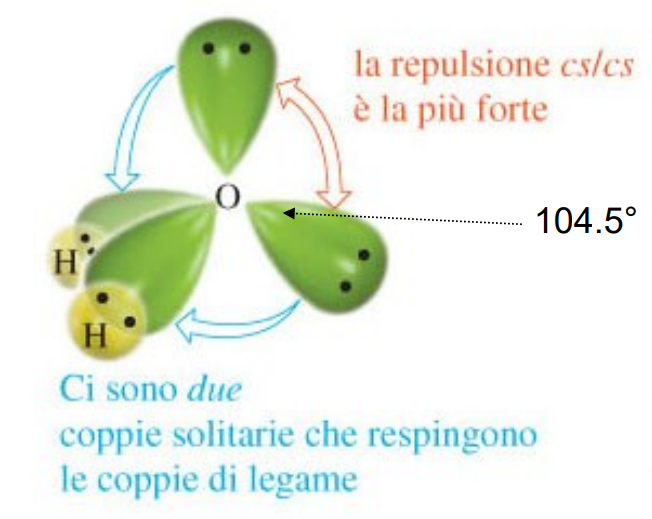
\includegraphics[width=6cm]{immagini/acqua.png}
    \end{figure}
\end{minipage}
\begin{minipage}{0.3\textwidth}
    \begin{figure}[H]
        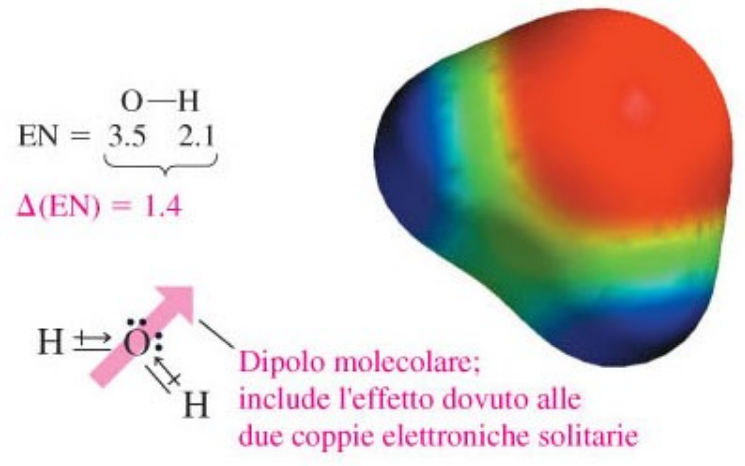
\includegraphics[width=5.5cm]{immagini/dipolo-acqua.png}
    \end{figure}
\end{minipage}

\vspace{0.2cm}Secondo il formalismo di Lewis, l'ossigeno dell'acqua ha attorno due coppie di legame e due solitarie. Anche qui immaginiamo che ci sia ibridizzazione sp$^3$, solo che stavolta due lobi saranno coinvolti nei legami idrogeno-ossigeno, gli altri due ospiteranno le coppie solitarie. Si parte quindi da un sistema tetraedrico, solo che stavolta ci aspettiamo degli angoli ancora più chiusi. Infatti sull'acqua si osservano angoli di 104.5°. Ciò, sempre sulla base della teoria V.S.E.P.R.\,, è ragionevole, perché stavolta ci sono due coppie solitarie, le quali fra loro si respingono molto di più in quanto giacciono su un solo atomo e quindi hanno meno spazio per delocalizzarsi, facendo chiudere maggiormente l'angolo idrogeno-ossigeno-idrogeno.

Quindi se considerassimo solo gli atomi di idrogeno e quello di ossigeno e le coppie di legame, diremmo che tale molecola è planare; se invece ragioniamo sulla geometria degli orbitali dell'ossigeno ci accorgiamo che non lo è, in quanto ci sono anche i due orbitali ibridi che ospitano le coppie solitarie.

Ricordiamo inoltre che l'ossigeno è fortemente elettronegativo rispetto all'idrogeno (3.5 contro 2.1), per cui la differenza in elettronegatività $\Delta EN$ è molto grande. Ne segue che sulla molecola la carica si delocalizza molto di più sull'ossigeno che sull'idrogeno. Tale fatto, unito alla presenza di coppie solitarie sull'ossigeno, rendono la molecola dipolare, cioè avente un momento di dipolo.

Ciò graficamente si rappresenta con una zona rossa indicante l'addensamento di elettroni, e con le zone blu che indicano la parziale carica positiva che si genera.

\subsection{Molecole planari}
\vspace{-0.4cm}
\begin{minipage}{0.4\textwidth}
    \begin{figure}[H]
        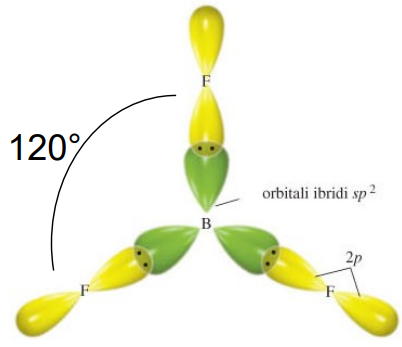
\includegraphics[width=5cm]{immagini/BF_3.png} 
    \end{figure}
\end{minipage}
\hfill
\begin{minipage}{0.6\textwidth}
\vspace{0.6cm}Consideriamo la molecola $\rm BF_3$. Contando gli elettroni, i tre atomi di fluoro forniscono 7 elettroni ciascuno quindi 21, più i 3 elettroni forniti dal boro arriviamo a 24. Spendiamo 6 elettroni  per formare 3 legami, ne restano 18 cioè 9 coppie, che suddividiamo in 3 coppie su ciascun fluoro, per cui non ne dovremo mettere sul boro.

La geometria che permette di minimizzare le repulsioni tra le tre coppie di legame è quella trigonale planare.

Se sul boro ci fossero state coppie solitarie questo discorso non sarebbe andato bene: la struttura non sarebbe stata planare.
\end{minipage}

\subsection{Molecole lineari}

\begin{minipage}{0.4\textwidth}
    \begin{figure}[H]
        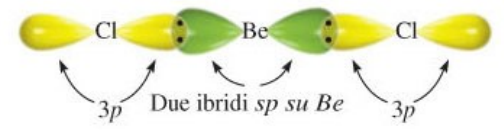
\includegraphics[width=6cm]{immagini/BeCl_2.png}
    \end{figure}
\end{minipage}
\hfill
\begin{minipage}{0.55\textwidth}
\vspace{0.4cm}Consideriamo la molecola $\rm BeCl_2$. Sul berillio non ci sono coppie solitarie ma ci sono due coppie di legame.

La geometria che rende minima la repulsione tra queste è quella lineare.
\end{minipage}

\subsection{Molecole con 5 coppie di elettroni}
\textbf{ES.1} $\rm PCl_5$ (5 coppie di legame)

\begin{minipage}{0.4\textwidth}
    \begin{figure}[H]
        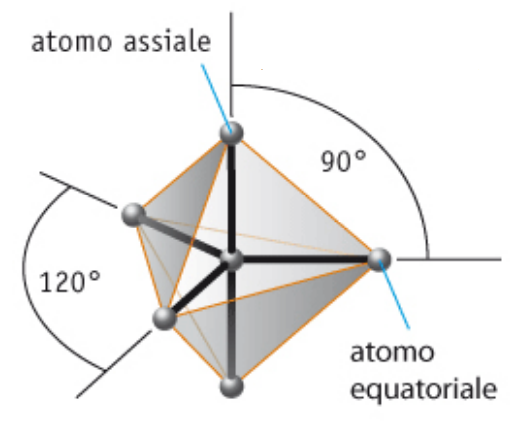
\includegraphics[width=6cm]{immagini/PCl_5.png}
    \end{figure}
\end{minipage}
\hfill
\begin{minipage}{0.55\textwidth}
    \vspace{0.2cm}Nel pentacloruro di fosforo, il fosforo centrale ha cinque legami. Per spiegare tale fatto tramite l'approccio di Lewis abbiamo introdotto il concetto di valenza espansa, dicendo che il fosforo dispone degli orbitali 3d vuoti, virtuali, che sono ad alta energia ma non così alta da non essere accessibili, perché hanno stesso numero quantico principale, e grazie ad essi il fosforo può ospitare nel suo intorno un numero di elettroni superiore ad 8.
\end{minipage}

\vspace{0.2cm}Per spiegare la geometria di tale molecola si va avanti sia con la teoria dell'ibridizzazione che con la teoria V.S.E.P.R.\,. Infatti si parla di ibridizzazione $\rm sp^3d$, cioè si aggiunge un quinto orbitale di tipo d. In questo modo riusciamo già a spiegare la geometria, che viene confermata dalla V.S.E.P.R.\,: non avendo coppie solitarie sul fosforo, il poliedro che tiene più lontane le cinque coppie di legame è la bipiramide a base triangolare.   

In essa il fosforo starà nel piano della base comune alle due piramidi, su cui ci sono anche 3 atomi di cloro distanti 120° l'uno dall'altro, che si dicono posti in posizione equatoriale. Gli altri due atomi di cloro giaceranno su un asse passante per il fosforo, perpendicolare alla base, per cui si dicono posti in posizione assiale.

\vspace{0.2cm}\textbf{ES.2} $\rm TeCl_4$ (4 coppie di legame e una solitaria)

\vspace{0.2cm}Nel momento in cui al posto delle coppie di legame abbiamo coppie solitarie, queste preferenzialmente andranno a sostituire atomi equatoriali.

\hspace{0.5cm}\begin{minipage}{0.2\textwidth}
    \begin{figure}[H]
        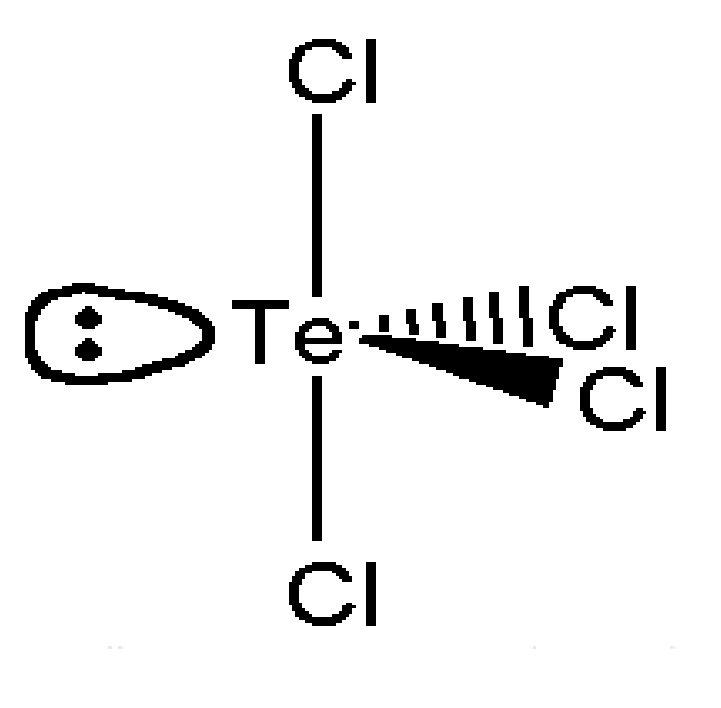
\includegraphics[width=4cm]{immagini/TeCl_4.png}
    \end{figure}
\end{minipage} \hfill
\begin{minipage}{0.65\textwidth}
    \vspace{0.4cm}
    Se quindi ad esempio avessimo un sistema con quattro coppie legate e una solitaria, questa andrebbe sul piano della base triangolare. È il caso del tetracloruro di tellurio.

    In esso un atomo della base è sostituito da una coppia solitaria, la quale respingerà maggiormente le coppie legate, facendo assumere alla molecola una geometria detta "ad altalena".
\end{minipage}

\vspace{0.3cm}\textbf{ES.3} $\rm ClF_3$ (3 coppie di legame e 2 solitarie)

\hspace{0.5cm}\begin{minipage}{0.2\textwidth}
    \begin{figure}[H]
        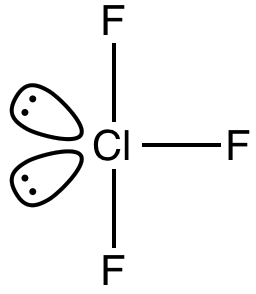
\includegraphics[width=3cm]{immagini/ClF_3.png}
    \end{figure}
\end{minipage} \hfill
\begin{minipage}{0.65\textwidth}
    \vspace{0.2cm}Se una seconda coppia solitaria va a sostituire un altro atomo in posizione equatoriale, come nel caso del trifluoruro di cloro, sul piano equatoriale si avranno ancora angoli di 120° e la geometria che viene fuori è detta "a T".
\end{minipage}

\vspace{0.2cm}\textbf{ES.4} $\rm I_3^-$ (2 coppie di legame e 3 solitarie)

\vspace{0.2cm}Se anche una terza coppia solitaria va a sostituire l'ultimo elettrone equatoriale, come nel caso dello ione triioduro, ci aspettiamo una geometria in cui le 3 coppie solitarie sono poste sul piano equatoriale a 120° l'una dall'altra e i 3 atomi di iodio allineati lungo l'asse. Questa molecola è quindi lineare:
$$
\chemleft[ \chemfig{\charge{[circle]90=\:,180=\:,270=\:}{I}-\charge{[circle]60=\:,120=\:,270=\:}{I}-\charge{[circle]0=\:,90=\:,270=\:}{I}} \chemright{]^{-}}
$$
Nota: le varie geometrie si ottengono considerando solo le coppie legate, se considerassimo anche le coppie solitarie la geometria sarebbe quella di una bipiramide a base triangolare in ogni caso.
\begin{figure}[htp]
    \centering
    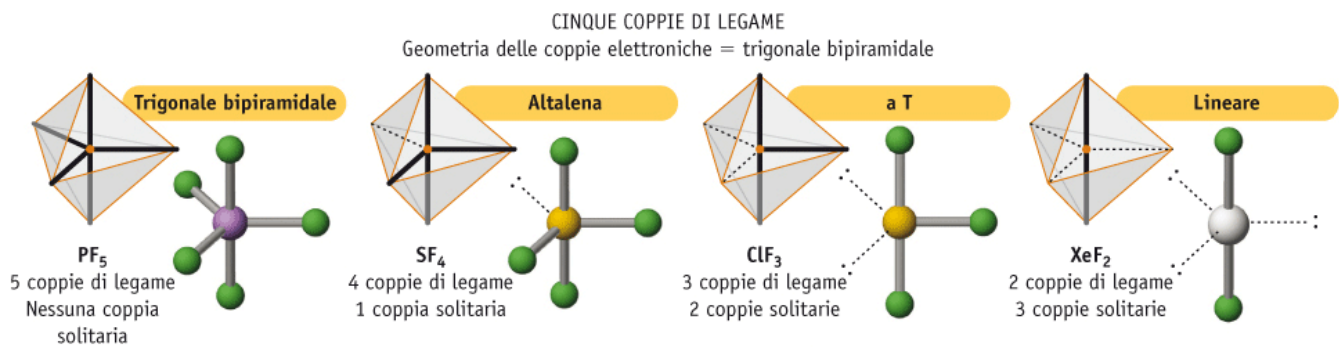
\includegraphics[width=14cm]{immagini/geometrie-5-coppie.png}
\end{figure}
\subsection{Molecole con 6 coppie di elettroni}
Per questi sistemi la teoria dell'ibridizzazione prevede il coinvolgimento di due orbitali d. Anche in questo caso avremo casi in cui ci sono più o meno coppie solitarie.

\vspace{0.2cm}\textbf{ES.1} $\rm SF_6$ (6 coppie di legame)

\hspace{1cm}\begin{minipage}{0.2\textwidth}
    \begin{figure}[H]
    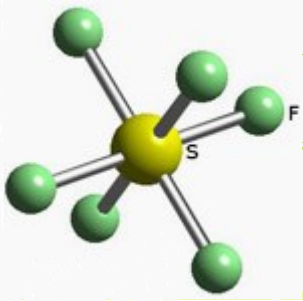
\includegraphics[width=3cm]{immagini/SF_6.png}
    \end{figure}
    \end{minipage} \hfill
    \begin{minipage}{0.65\textwidth}
        \vspace{0.2cm}Un esempio di questo tipo di sistemi è l'esafluoruro di zolfo. La geometria che permette di rendere minime le repulsioni tra le sue sei coppie legate è quella della struttura ottaedrica, cioè una bipiramide a base quadrata, quindi sul piano equatoriale ci saranno quattro vertici tutti alla stessa distanza, per cui le varie facce triangolari saranno tutte uguali.
    \end{minipage}

\vspace{0.2cm}\textbf{ES.2} $\rm IF_5$ (5 coppie di legame e una solitaria)

\hspace{0.5cm}\begin{minipage}{0.2\textwidth}
    \begin{figure}[H]
    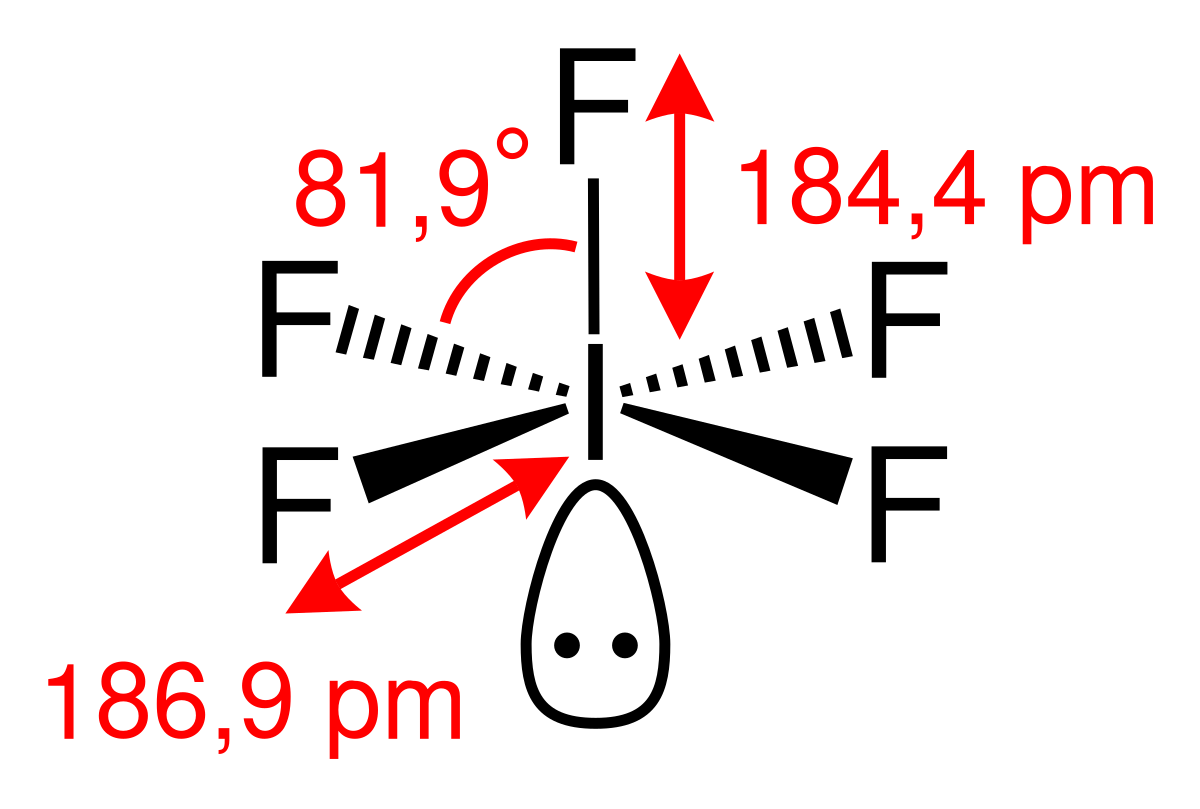
\includegraphics[width=4cm]{immagini/IF_5.png}
    \end{figure}
    \end{minipage} \hfill
    \begin{minipage}{0.65\textwidth}
        \vspace{0.2cm}Se sostituiamo una delle coppie legate con una solitaria, essa andrà a disporsi in posizione assiale. Ne è un esempio il pentafluoruro di iodio. Per tale molecola la geometria è quella di una "piramide a base quadrata", in cui lo iodio non giace sul piano della base.
    \end{minipage}

\vspace{0.2cm}\textbf{ES.3} ICl$_4^-$ (4 coppie di legame e due solitarie)

\hspace{0.5cm}\begin{minipage}{0.2\textwidth}
    \begin{figure}[H]
    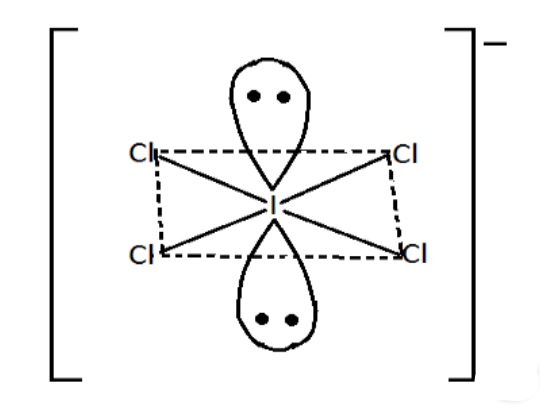
\includegraphics[width=4cm]{immagini/ICl_4.png}
    \end{figure}
    \end{minipage} \hfill
    \begin{minipage}{0.65\textwidth}
        \vspace{0.2cm}Se sostituiamo anche una seconda coppia legata con una coppia solitaria, la repulsione respingerà l'atomo centrale di nuovo sul piano equatoriale e la molecola avrà una geometria planare quadrata. Ne è un esempio lo ione $\rm ICl_4^-$.
    \end{minipage}

\vspace{0.2cm}Nota: le varie geometrie si ottengono considerando solo le coppie legate, se considerassimo anche le coppi solitarie la geometria sarebbe quella di una bipiramide a base quadrata in ogni caso.

\begin{figure}[htp]
    \centering
    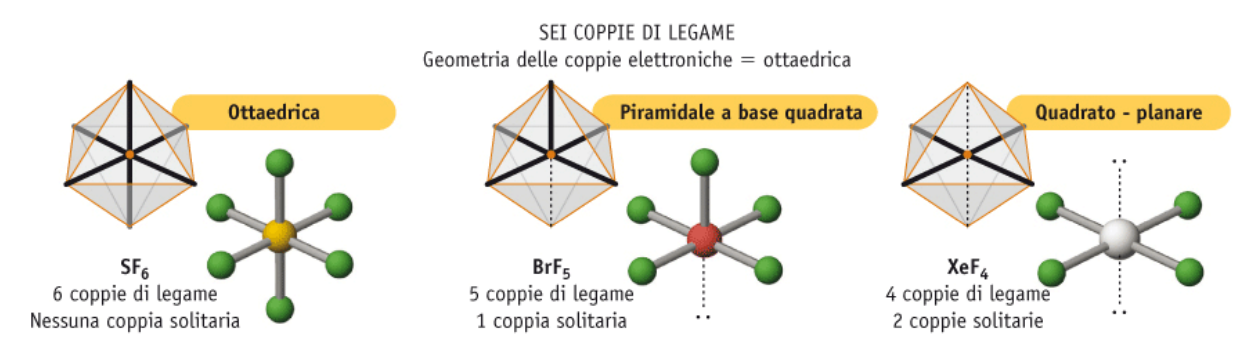
\includegraphics[width=14cm]{immagini/geometrie-6-coppie.png}
\end{figure}